\documentclass[a4paper, 12pt]{article}
\usepackage[left = 13 mm, top = 15mm, right = 13 mm, bottom = 23mm, bindingoffset = 7mm]{geometry}
\usepackage[T2A,T1]{fontenc}
\usepackage[utf8]{inputenc}
\usepackage[english,russian]{babel}
\usepackage{graphicx}
\usepackage{amssymb, mathtools}
\usepackage{lipsum}
\usepackage{float}
\usepackage{wrapfig}
\usepackage{indentfirst} 

\newcommand{\HRule}{\rule{\linewidth}{0.3mm}}

\newcommand{\LabTitle}{Гармонический анализ}
\begin{document}

\begin{titlepage}
\begin{center}\large
ФГАУ ВПО <<МОСКОВСКИЙ ФИЗИКО-ТЕХНИЧЕСКИЙ УНИВЕРСИТЕТ>>
\begin{figure}[H]
\centering

\includegraphics[width=15cm]{logo.jpg}
\end{figure}
{\Large
Кафедра радиотехники}

\vfill

\hrule
\vspace{0.3cm}

\huge \LabTitle

\vspace{0.3cm}
\hrule


%\noindent\rule{\textwidth}{0.4mm}
%\huge Магнитометр
%\noindent\rule{\textwidth}{0.4mm}


\end{center}

\vfill


\begin{minipage}{0.7\textwidth}
\textbf{Выполнил:}
Корепанов Г.М.

512 группа

\vspace{0.5cm}

\textbf{Преподаватель:}
Филатов Иван Васильевич
\end{minipage}


\vfill
\centering
 Долгопрудный, 2016 г.




\end{titlepage}

\section{Цель работы}

Изучить спектральный состав периодических электрических сигналов различной формы: последовательности прямоугольных импульсов, последовательности цугов и амплитудно - модулированных гармонических колебаний.

\section{Теоретический материал}

\subsection{Спектральный анализ}

Рассмотрим функцию вида:
$$f(t) = A_{1}cos(\omega_1t-\alpha_{1}) + ... + A_{n}cos(\omega_{n}t-\alpha_{n})$$
или, что то же самое:
$$f(t) = \sum\limits_{i=1}^n A_{i}cos(\omega_{i}t-\alpha_{i})$$
Причем, $A_{i}, \omega_{i}, \alpha_{i}$ - постоянные константы. Множество пар $(\omega_{i}, A_{i}), \: i \in 1..N$ - называется спектром функции $f(t)$.

\subsection{Периодические сигналы}

Часто встречаемая задача - разложение сложного сигнала на гармонические колебания различных частот $\omega$. Представление периодического сигнала в виде суммы гармонических сигналов называется {\it{разложением в ряд Фурье}}.

Пусть заданная функция $f(t)$ - периодически повторяется с частотой $\Omega_{1}=\frac{2\pi}{T}$, где $T$ - период повторения сигнала $f(t)$
Её разложение в ряд Фурье имеет вид:
\begin{equation}
\label{form:furie}	
	f(t)=\frac{a_{0}}{2}+\sum\limits_{n=1}^{\infty}a_{n}\cos(n\Omega_{1}t)+b_{n}\sin(n\Omega_{1}t) 
\end{equation}

или
\begin{equation}
	f(t)=\frac{a_{0}}{2}+\sum\limits_{n=1}^{\infty}A_{n}\cos(n\Omega_{1}t-\psi_{n}) 
\label{form:furie_2}
\end{equation}

где $\frac{a_{0}}{2}$ - среднее значение функции $f(t)$. Постоянные $a_n$ и $b_n$ определяются выражениями:
\begin{equation}
\label{form:a_n}
	a_{n} = \frac{2}{T}\int\limits_{t_{1}}^{t_{1}+T}f(t)\cos(n\Omega_1t)\, dt
\end{equation}

\begin{equation}
	b_{n} = \frac{2}{T}\int\limits_{t_{1}}^{t_{1}+T}f(t)\sin(n\Omega_{1}t)\, dt 
\label{form:b_n}
\end{equation}

причем точку $t_{1}$ можно выбрать любую.

\begin{equation}
\label{form:A_n}
	A_{n} = \sqrt{a_{n}^2+b_{n}^2}
\end{equation}
\begin{equation}
	\psi_{n} = \arctan\frac{b_{n}}{a_{n}}
\label{form:psi_n}
\end{equation}
\section{Работа и измерения}
\subsection*{Исследование спектра периодической последовательности прямоугольных импульсов}

$V_0$  - амплитуда, $\tau$ - длительность, $f_\text{повт} = \frac{2\pi}{T} $ - частота повторения.

Согласно формуле \ref{form:a_n} находим:
$$ \langle V \rangle = \frac{a_0}{2} =  \frac{1}{T}\int\limits_{ -\frac{\tau}{2} } ^ {\frac{\tau}{2} } V_0\,dt = V_0 \frac{\tau}{T}
$$
\begin{equation}
\label{form:app_a_n}
	a_n = \frac{2}{T}\int\limits_{ -\frac{\tau}{2} } ^ {\frac{\tau}{2} } V_0\cos(nf_\text{повт}t)\, dt \sim \frac{\sin(x)}{x}
\end{equation}
 
В силу чётности функции $\forall n \in {N} \ b_n=0$. Таким образом, спектр периодической последовательности прямоугольных импульсов должен выглядеть как график $\frac{\sin(x)}{x}$.
\subsubsection*{Работа}
В работе используются: \textit{анализатор спектра СК4-56; генератор прямоугольных импульсов Г5-54; осциллограф}



\begin{figure}[H]
\centering
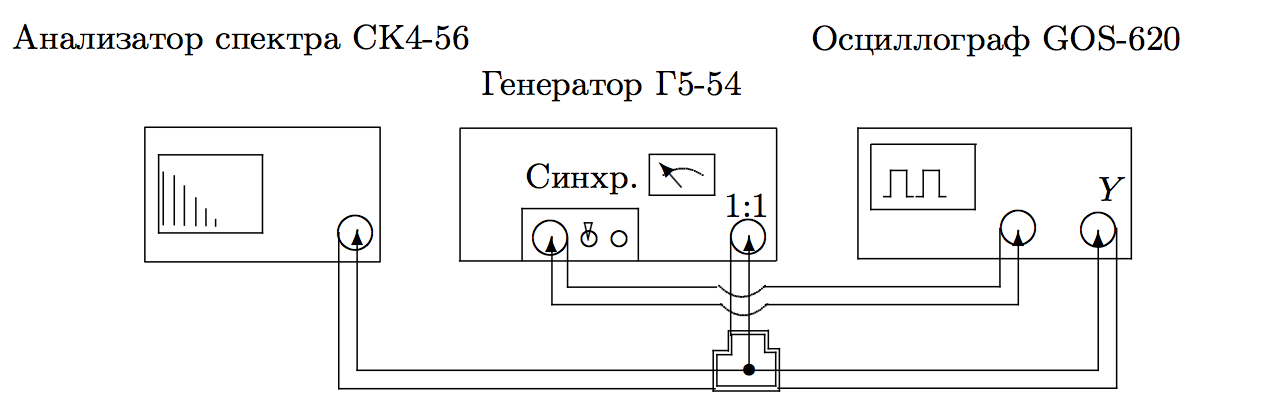
\includegraphics[width = 0.8\textwidth]{SchemeA}
\caption{Схема для исследования спектра периодической последовательности прямоугольных импульсов}
\label{img:scheme A}
\end{figure}

Собираем схему согласно \ref{img:scheme A}. Получаем на экране осциллографа последовательность периодических прямоугольных импульсов. Подключаем анализатор спектра СК4-56 и после настройки наблюдаем спектр сигнала с параметрами: $$f_\text{повт} = 10^3 \; \text{Гц}, \tau = 25 \; \text{мкс}, m_x = 5 \; \text{кГц}$$

При увеличении частоты повторений $f_\text{повт}$ вдвое при неизменном $\tau$, увеличивается расстояние $\delta \nu$. При увеличении $\tau$ вдвое при неизменной частоте повторений, уменьшается ширина спектра, в соответствии с соотношением неопределенности: $\Delta \nu \tau \simeq 1$.

\subsubsection*{Измерения}
$$\sigma \Delta \nu = 2.5 \; \text{кГц}$$
\begin{table}[H]
\centering
\begin{tabular}{|l|l|l|l|l|l|l|l|l|l|}
\hline
\textbf{$\tau, \text{мкс}$}       & 150          & 125 & 100 & 80   & 50 & 40 & 30            & 25 & 20 \\ \hline
\textbf{$\Delta \nu, \text{кГц}$} & 7            & 8.5 & 10  & 12.5 & 19 & 23 & 34            & 41 & 50 \\ \hline
\textbf{$1/\tau, \text{кГц}$}     & 7 & 8   & 10  & 12.5 & 20 & 25 & 33 & 40 & 50 \\ \hline
\end{tabular}
\caption{Зависимость ширины $\Delta \nu$ спектра  от длительности импульса $\tau$}
\label{my-label}
\end{table}


\begin {figure}[H]
\begin{center}
{% GNUPLOT: LaTeX picture with Postscript
\begingroup
  \fontfamily{sansserif}%
  \selectfont
  \makeatletter
  \providecommand\color[2][]{%
    \GenericError{(gnuplot) \space\space\space\@spaces}{%
      Package color not loaded in conjunction with
      terminal option `colourtext'%
    }{See the gnuplot documentation for explanation.%
    }{Either use 'blacktext' in gnuplot or load the package
      color.sty in LaTeX.}%
    \renewcommand\color[2][]{}%
  }%
  \providecommand\includegraphics[2][]{%
    \GenericError{(gnuplot) \space\space\space\@spaces}{%
      Package graphicx or graphics not loaded%
    }{See the gnuplot documentation for explanation.%
    }{The gnuplot epslatex terminal needs graphicx.sty or graphics.sty.}%
    \renewcommand\includegraphics[2][]{}%
  }%
  \providecommand\rotatebox[2]{#2}%
  \@ifundefined{ifGPcolor}{%
    \newif\ifGPcolor
    \GPcolorfalse
  }{}%
  \@ifundefined{ifGPblacktext}{%
    \newif\ifGPblacktext
    \GPblacktexttrue
  }{}%
  % define a \g@addto@macro without @ in the name:
  \let\gplgaddtomacro\g@addto@macro
  % define empty templates for all commands taking text:
  \gdef\gplbacktext{}%
  \gdef\gplfronttext{}%
  \makeatother
  \ifGPblacktext
    % no textcolor at all
    \def\colorrgb#1{}%
    \def\colorgray#1{}%
  \else
    % gray or color?
    \ifGPcolor
      \def\colorrgb#1{\color[rgb]{#1}}%
      \def\colorgray#1{\color[gray]{#1}}%
      \expandafter\def\csname LTw\endcsname{\color{white}}%
      \expandafter\def\csname LTb\endcsname{\color{black}}%
      \expandafter\def\csname LTa\endcsname{\color{black}}%
      \expandafter\def\csname LT0\endcsname{\color[rgb]{1,0,0}}%
      \expandafter\def\csname LT1\endcsname{\color[rgb]{0,1,0}}%
      \expandafter\def\csname LT2\endcsname{\color[rgb]{0,0,1}}%
      \expandafter\def\csname LT3\endcsname{\color[rgb]{1,0,1}}%
      \expandafter\def\csname LT4\endcsname{\color[rgb]{0,1,1}}%
      \expandafter\def\csname LT5\endcsname{\color[rgb]{1,1,0}}%
      \expandafter\def\csname LT6\endcsname{\color[rgb]{0,0,0}}%
      \expandafter\def\csname LT7\endcsname{\color[rgb]{1,0.3,0}}%
      \expandafter\def\csname LT8\endcsname{\color[rgb]{0.5,0.5,0.5}}%
    \else
      % gray
      \def\colorrgb#1{\color{black}}%
      \def\colorgray#1{\color[gray]{#1}}%
      \expandafter\def\csname LTw\endcsname{\color{white}}%
      \expandafter\def\csname LTb\endcsname{\color{black}}%
      \expandafter\def\csname LTa\endcsname{\color{black}}%
      \expandafter\def\csname LT0\endcsname{\color{black}}%
      \expandafter\def\csname LT1\endcsname{\color{black}}%
      \expandafter\def\csname LT2\endcsname{\color{black}}%
      \expandafter\def\csname LT3\endcsname{\color{black}}%
      \expandafter\def\csname LT4\endcsname{\color{black}}%
      \expandafter\def\csname LT5\endcsname{\color{black}}%
      \expandafter\def\csname LT6\endcsname{\color{black}}%
      \expandafter\def\csname LT7\endcsname{\color{black}}%
      \expandafter\def\csname LT8\endcsname{\color{black}}%
    \fi
  \fi
    \setlength{\unitlength}{0.0500bp}%
    \ifx\gptboxheight\undefined%
      \newlength{\gptboxheight}%
      \newlength{\gptboxwidth}%
      \newsavebox{\gptboxtext}%
    \fi%
    \setlength{\fboxrule}{0.5pt}%
    \setlength{\fboxsep}{1pt}%
\begin{picture}(9354.00,6802.00)%
    \gplgaddtomacro\gplbacktext{%
      \csname LTb\endcsname%
      \put(660,1408){\makebox(0,0)[r]{\strut{}$0$}}%
      \csname LTb\endcsname%
      \put(660,2381){\makebox(0,0)[r]{\strut{}$10$}}%
      \csname LTb\endcsname%
      \put(660,3354){\makebox(0,0)[r]{\strut{}$20$}}%
      \csname LTb\endcsname%
      \put(660,4327){\makebox(0,0)[r]{\strut{}$30$}}%
      \csname LTb\endcsname%
      \put(660,5300){\makebox(0,0)[r]{\strut{}$40$}}%
      \csname LTb\endcsname%
      \put(660,6273){\makebox(0,0)[r]{\strut{}$50$}}%
      \csname LTb\endcsname%
      \put(924,968){\makebox(0,0){\strut{}$0$}}%
      \csname LTb\endcsname%
      \put(2604,968){\makebox(0,0){\strut{}$10$}}%
      \csname LTb\endcsname%
      \put(4285,968){\makebox(0,0){\strut{}$20$}}%
      \csname LTb\endcsname%
      \put(5965,968){\makebox(0,0){\strut{}$30$}}%
      \csname LTb\endcsname%
      \put(7646,968){\makebox(0,0){\strut{}$40$}}%
      \csname LTb\endcsname%
      \put(9326,968){\makebox(0,0){\strut{}$50$}}%
      \put(1764,5787){\makebox(0,0)[l]{\strut{}$K = \left(0.99\pm0.02\right)$ }}%
    }%
    \gplgaddtomacro\gplfronttext{%
      \csname LTb\endcsname%
      \put(44,3840){\rotatebox{-270}{\makebox(0,0){\strut{}$1/\tau$, кГц}}}%
      \put(5125,308){\makebox(0,0){\strut{}$\Delta \nu$, кГц}}%
    }%
    \gplbacktext
    \put(0,0){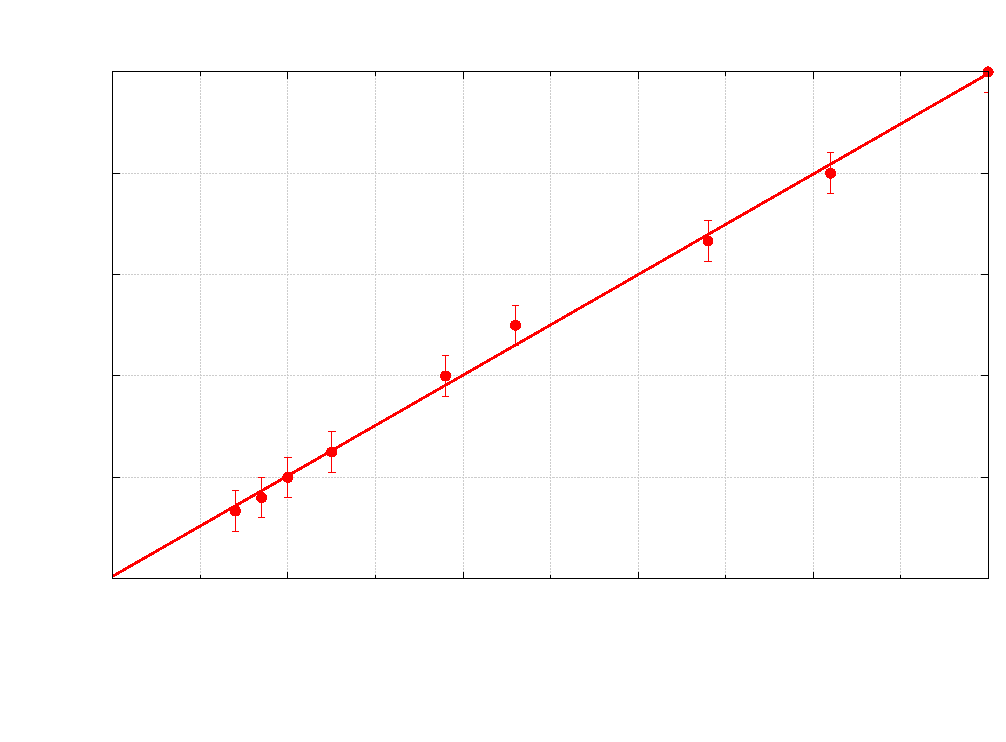
\includegraphics{nutau}}%
    \gplfronttext
  \end{picture}%
\endgroup
}
\caption{График зависимости $\Delta \nu (\frac{1}{\tau})$}
\end{center}
\end{figure}


Коэффициент угла наклона прямой и его погрешность посчитаем методом наименьших квадратов: $\Delta k = \Delta(\nu \tau) = 0,99 \pm 0,05$

\begin{figure}[H]
\begin{minipage}[h]{0.49\linewidth}
\center{\includegraphics[width=0.9\linewidth]{1ex} \\ $\tau = 50$ мкс}
\end{minipage}
\hfill
\begin{minipage}[h]{0.49\linewidth}
\center{\includegraphics[width=0.9\linewidth]{2ex} \\ $\tau = 100$ мкс}
\end{minipage}
\caption{Спектры колебаний с различными параметрами длительности импульса}
\label{ris:image1}
\end{figure}


\subsection*{Исследование спектра периодической последовательности цугов \\ гармонических колебаний}

Рассмотрим периодическую последовательность {\it{цугов}} гармонического колебания \\
$V_0 \cos (\omega_0 t)$ c длительностью цуга $\tau$.
Тогда согласно \ref{form:a_n}:

\begin{equation}
\label{form:cug_a_n}
a_n = \frac{2}{T}\int\limits_{ -\frac{\tau}{2} } ^ {\frac{\tau}{2} } V_0\cos(\omega_0t)\cdot \cos(n\Omega_1)\, dt
\end{equation}

\subsubsection*{Работа}

В работе используются: \textit{анализатор спектра СК4-56; генератор прямоугольных импульсов Г5-54; осциллограф; генератор сигналов Г6-34}

\begin{figure}[H]
\centering
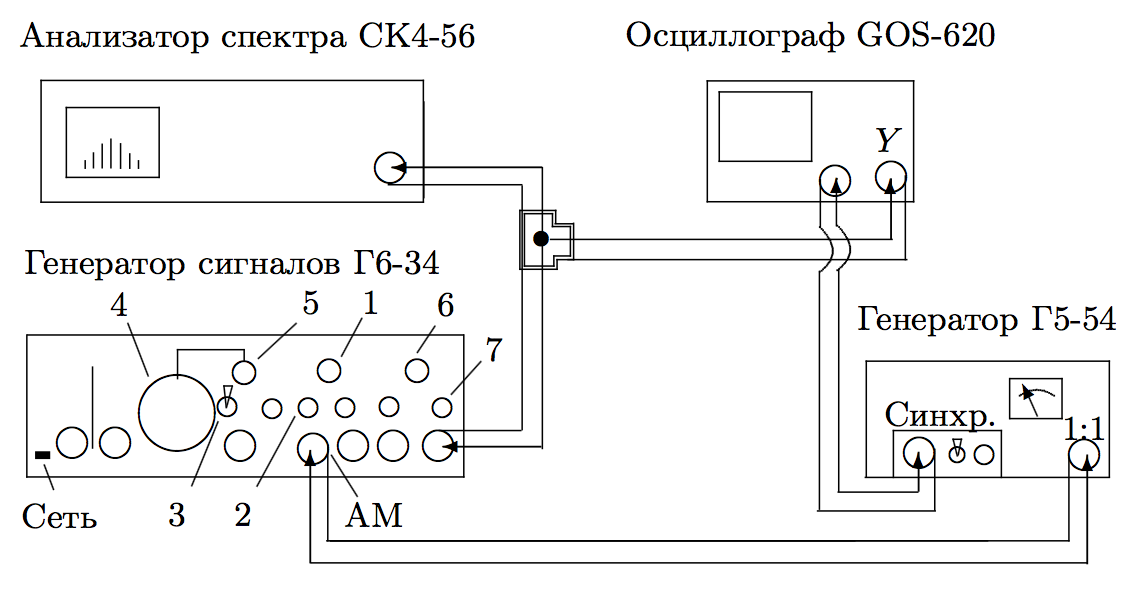
\includegraphics[width = 0.8\textwidth]{SchemeB}
\caption{Схема для исследования спектра периодической последовательности цугов высокочастотных колебаний}
\label{img:scheme B}
\end{figure}

Собираем схему согласно \ref{img:scheme B}. Получаем на экране осциллографа последовательность периодических цугов гармонических колебаний, получаемых модулированием синусоиды прямоугольными импульсами. Подключаем анализатор спектра СК4-56 и после настройки наблюдаем спектр сигнала с параметрами: $$ \nu_0 = 25 \; \text{кГц}, f_\text{повт} = 10^3 \; \text{Гц}, \tau = 100 \; \text{мкс}, m_x = 5 \; \text{кГц}$$

При увеличении $\tau$ вдвое при неизменной частоте повторений, вдвое уменьшается ширина спектра, в соответствии с соотношением неопределенности: $\Delta \nu \tau \simeq 1$.

При изменении несущей частоты  $\nu_0 = 25, 10 \; \text{или} \; 40\; \text{кГц}$ при неизменных $f_\text{повт} = 10^3 \; \text{Гц}, \tau = 100 \; \text{мкс}, m_x = 5 \; \text{кГц}$, изменяется сдвиг спектра по оси частот.

\begin{table}[H]
\centering
\begin{tabular}{|l|l|l|l|l|l|}
\hline
\textbf{$\delta \nu$, кГц}    & 30 & 15 & 11  & 20  & 12  \\ \hline
\textbf{$N$}                  & 30 & 30 & 30  & 30  & 30  \\ \hline
\textbf{$\nu$, кГц}           & 1  & 2  & 2.7 & 1.5 & 2.5 \\ \hline
\textbf{$f_\text{повт}$, кГц} & 1  & 2  & 2.7 & 1.5 & 2.5 \\ \hline
\end{tabular}
\caption{Зависимость расстояния между соседними спектральными компонентами от $f_\text{повт}$ при $\tau = 50 \text{ мкс}$ }
\label{my-label}
\end{table}

\begin {figure}[H]
\begin{center}
{% GNUPLOT: LaTeX picture with Postscript
\begingroup
  \fontfamily{sansserif}%
  \selectfont
  \makeatletter
  \providecommand\color[2][]{%
    \GenericError{(gnuplot) \space\space\space\@spaces}{%
      Package color not loaded in conjunction with
      terminal option `colourtext'%
    }{See the gnuplot documentation for explanation.%
    }{Either use 'blacktext' in gnuplot or load the package
      color.sty in LaTeX.}%
    \renewcommand\color[2][]{}%
  }%
  \providecommand\includegraphics[2][]{%
    \GenericError{(gnuplot) \space\space\space\@spaces}{%
      Package graphicx or graphics not loaded%
    }{See the gnuplot documentation for explanation.%
    }{The gnuplot epslatex terminal needs graphicx.sty or graphics.sty.}%
    \renewcommand\includegraphics[2][]{}%
  }%
  \providecommand\rotatebox[2]{#2}%
  \@ifundefined{ifGPcolor}{%
    \newif\ifGPcolor
    \GPcolorfalse
  }{}%
  \@ifundefined{ifGPblacktext}{%
    \newif\ifGPblacktext
    \GPblacktexttrue
  }{}%
  % define a \g@addto@macro without @ in the name:
  \let\gplgaddtomacro\g@addto@macro
  % define empty templates for all commands taking text:
  \gdef\gplbacktext{}%
  \gdef\gplfronttext{}%
  \makeatother
  \ifGPblacktext
    % no textcolor at all
    \def\colorrgb#1{}%
    \def\colorgray#1{}%
  \else
    % gray or color?
    \ifGPcolor
      \def\colorrgb#1{\color[rgb]{#1}}%
      \def\colorgray#1{\color[gray]{#1}}%
      \expandafter\def\csname LTw\endcsname{\color{white}}%
      \expandafter\def\csname LTb\endcsname{\color{black}}%
      \expandafter\def\csname LTa\endcsname{\color{black}}%
      \expandafter\def\csname LT0\endcsname{\color[rgb]{1,0,0}}%
      \expandafter\def\csname LT1\endcsname{\color[rgb]{0,1,0}}%
      \expandafter\def\csname LT2\endcsname{\color[rgb]{0,0,1}}%
      \expandafter\def\csname LT3\endcsname{\color[rgb]{1,0,1}}%
      \expandafter\def\csname LT4\endcsname{\color[rgb]{0,1,1}}%
      \expandafter\def\csname LT5\endcsname{\color[rgb]{1,1,0}}%
      \expandafter\def\csname LT6\endcsname{\color[rgb]{0,0,0}}%
      \expandafter\def\csname LT7\endcsname{\color[rgb]{1,0.3,0}}%
      \expandafter\def\csname LT8\endcsname{\color[rgb]{0.5,0.5,0.5}}%
    \else
      % gray
      \def\colorrgb#1{\color{black}}%
      \def\colorgray#1{\color[gray]{#1}}%
      \expandafter\def\csname LTw\endcsname{\color{white}}%
      \expandafter\def\csname LTb\endcsname{\color{black}}%
      \expandafter\def\csname LTa\endcsname{\color{black}}%
      \expandafter\def\csname LT0\endcsname{\color{black}}%
      \expandafter\def\csname LT1\endcsname{\color{black}}%
      \expandafter\def\csname LT2\endcsname{\color{black}}%
      \expandafter\def\csname LT3\endcsname{\color{black}}%
      \expandafter\def\csname LT4\endcsname{\color{black}}%
      \expandafter\def\csname LT5\endcsname{\color{black}}%
      \expandafter\def\csname LT6\endcsname{\color{black}}%
      \expandafter\def\csname LT7\endcsname{\color{black}}%
      \expandafter\def\csname LT8\endcsname{\color{black}}%
    \fi
  \fi
    \setlength{\unitlength}{0.0500bp}%
    \ifx\gptboxheight\undefined%
      \newlength{\gptboxheight}%
      \newlength{\gptboxwidth}%
      \newsavebox{\gptboxtext}%
    \fi%
    \setlength{\fboxrule}{0.5pt}%
    \setlength{\fboxsep}{1pt}%
\begin{picture}(9354.00,6802.00)%
    \gplgaddtomacro\gplbacktext{%
      \csname LTb\endcsname%
      \put(660,1408){\makebox(0,0)[r]{\strut{}$0$}}%
      \csname LTb\endcsname%
      \put(660,2277){\makebox(0,0)[r]{\strut{}$0.5$}}%
      \csname LTb\endcsname%
      \put(660,3146){\makebox(0,0)[r]{\strut{}$1$}}%
      \csname LTb\endcsname%
      \put(660,4014){\makebox(0,0)[r]{\strut{}$1.5$}}%
      \csname LTb\endcsname%
      \put(660,4883){\makebox(0,0)[r]{\strut{}$2$}}%
      \csname LTb\endcsname%
      \put(660,5752){\makebox(0,0)[r]{\strut{}$2.5$}}%
      \csname LTb\endcsname%
      \put(924,968){\makebox(0,0){\strut{}$0$}}%
      \csname LTb\endcsname%
      \put(2424,968){\makebox(0,0){\strut{}$0.5$}}%
      \csname LTb\endcsname%
      \put(3925,968){\makebox(0,0){\strut{}$1$}}%
      \csname LTb\endcsname%
      \put(5425,968){\makebox(0,0){\strut{}$1.5$}}%
      \csname LTb\endcsname%
      \put(6925,968){\makebox(0,0){\strut{}$2$}}%
      \csname LTb\endcsname%
      \put(8426,968){\makebox(0,0){\strut{}$2.5$}}%
      \csname LTb\endcsname%
      \put(1764,5787){\makebox(0,0)[l]{\strut{}$K = \left(1.01\pm0.08\right)$ }}%
    }%
    \gplgaddtomacro\gplfronttext{%
      \csname LTb\endcsname%
      \put(-220,3840){\rotatebox{-270}{\makebox(0,0){\strut{}$\delta f$, кГц}}}%
      \put(5125,308){\makebox(0,0){\strut{}$f_\text{повт}$, кГц}}%
    }%
    \gplbacktext
    \put(0,0){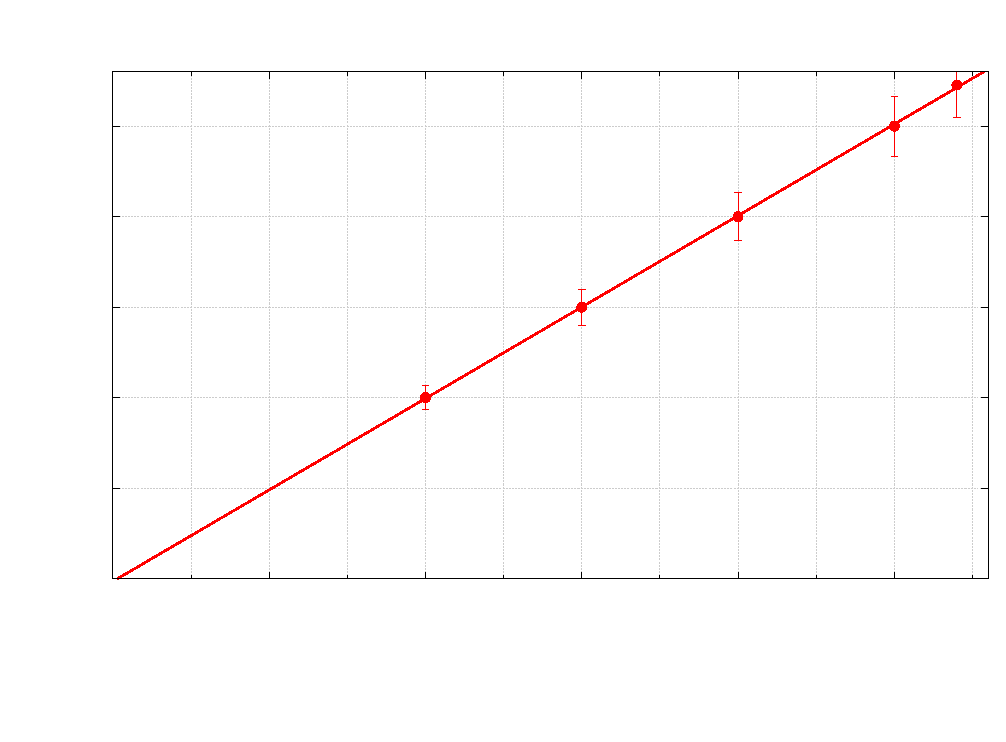
\includegraphics{deltaf}}%
    \gplfronttext
  \end{picture}%
\endgroup
}
\caption{График зависимости $\delta \nu (f_\text{повт})$}
\end{center}
\end{figure}



Коэффициент угла наклона прямой и его погрешность посчитаем методом наименьших квадратов: $K = \left(1.01\pm0.08\right)$.


\begin{figure}[H]
\begin{minipage}[h]{0.49\linewidth}
\center{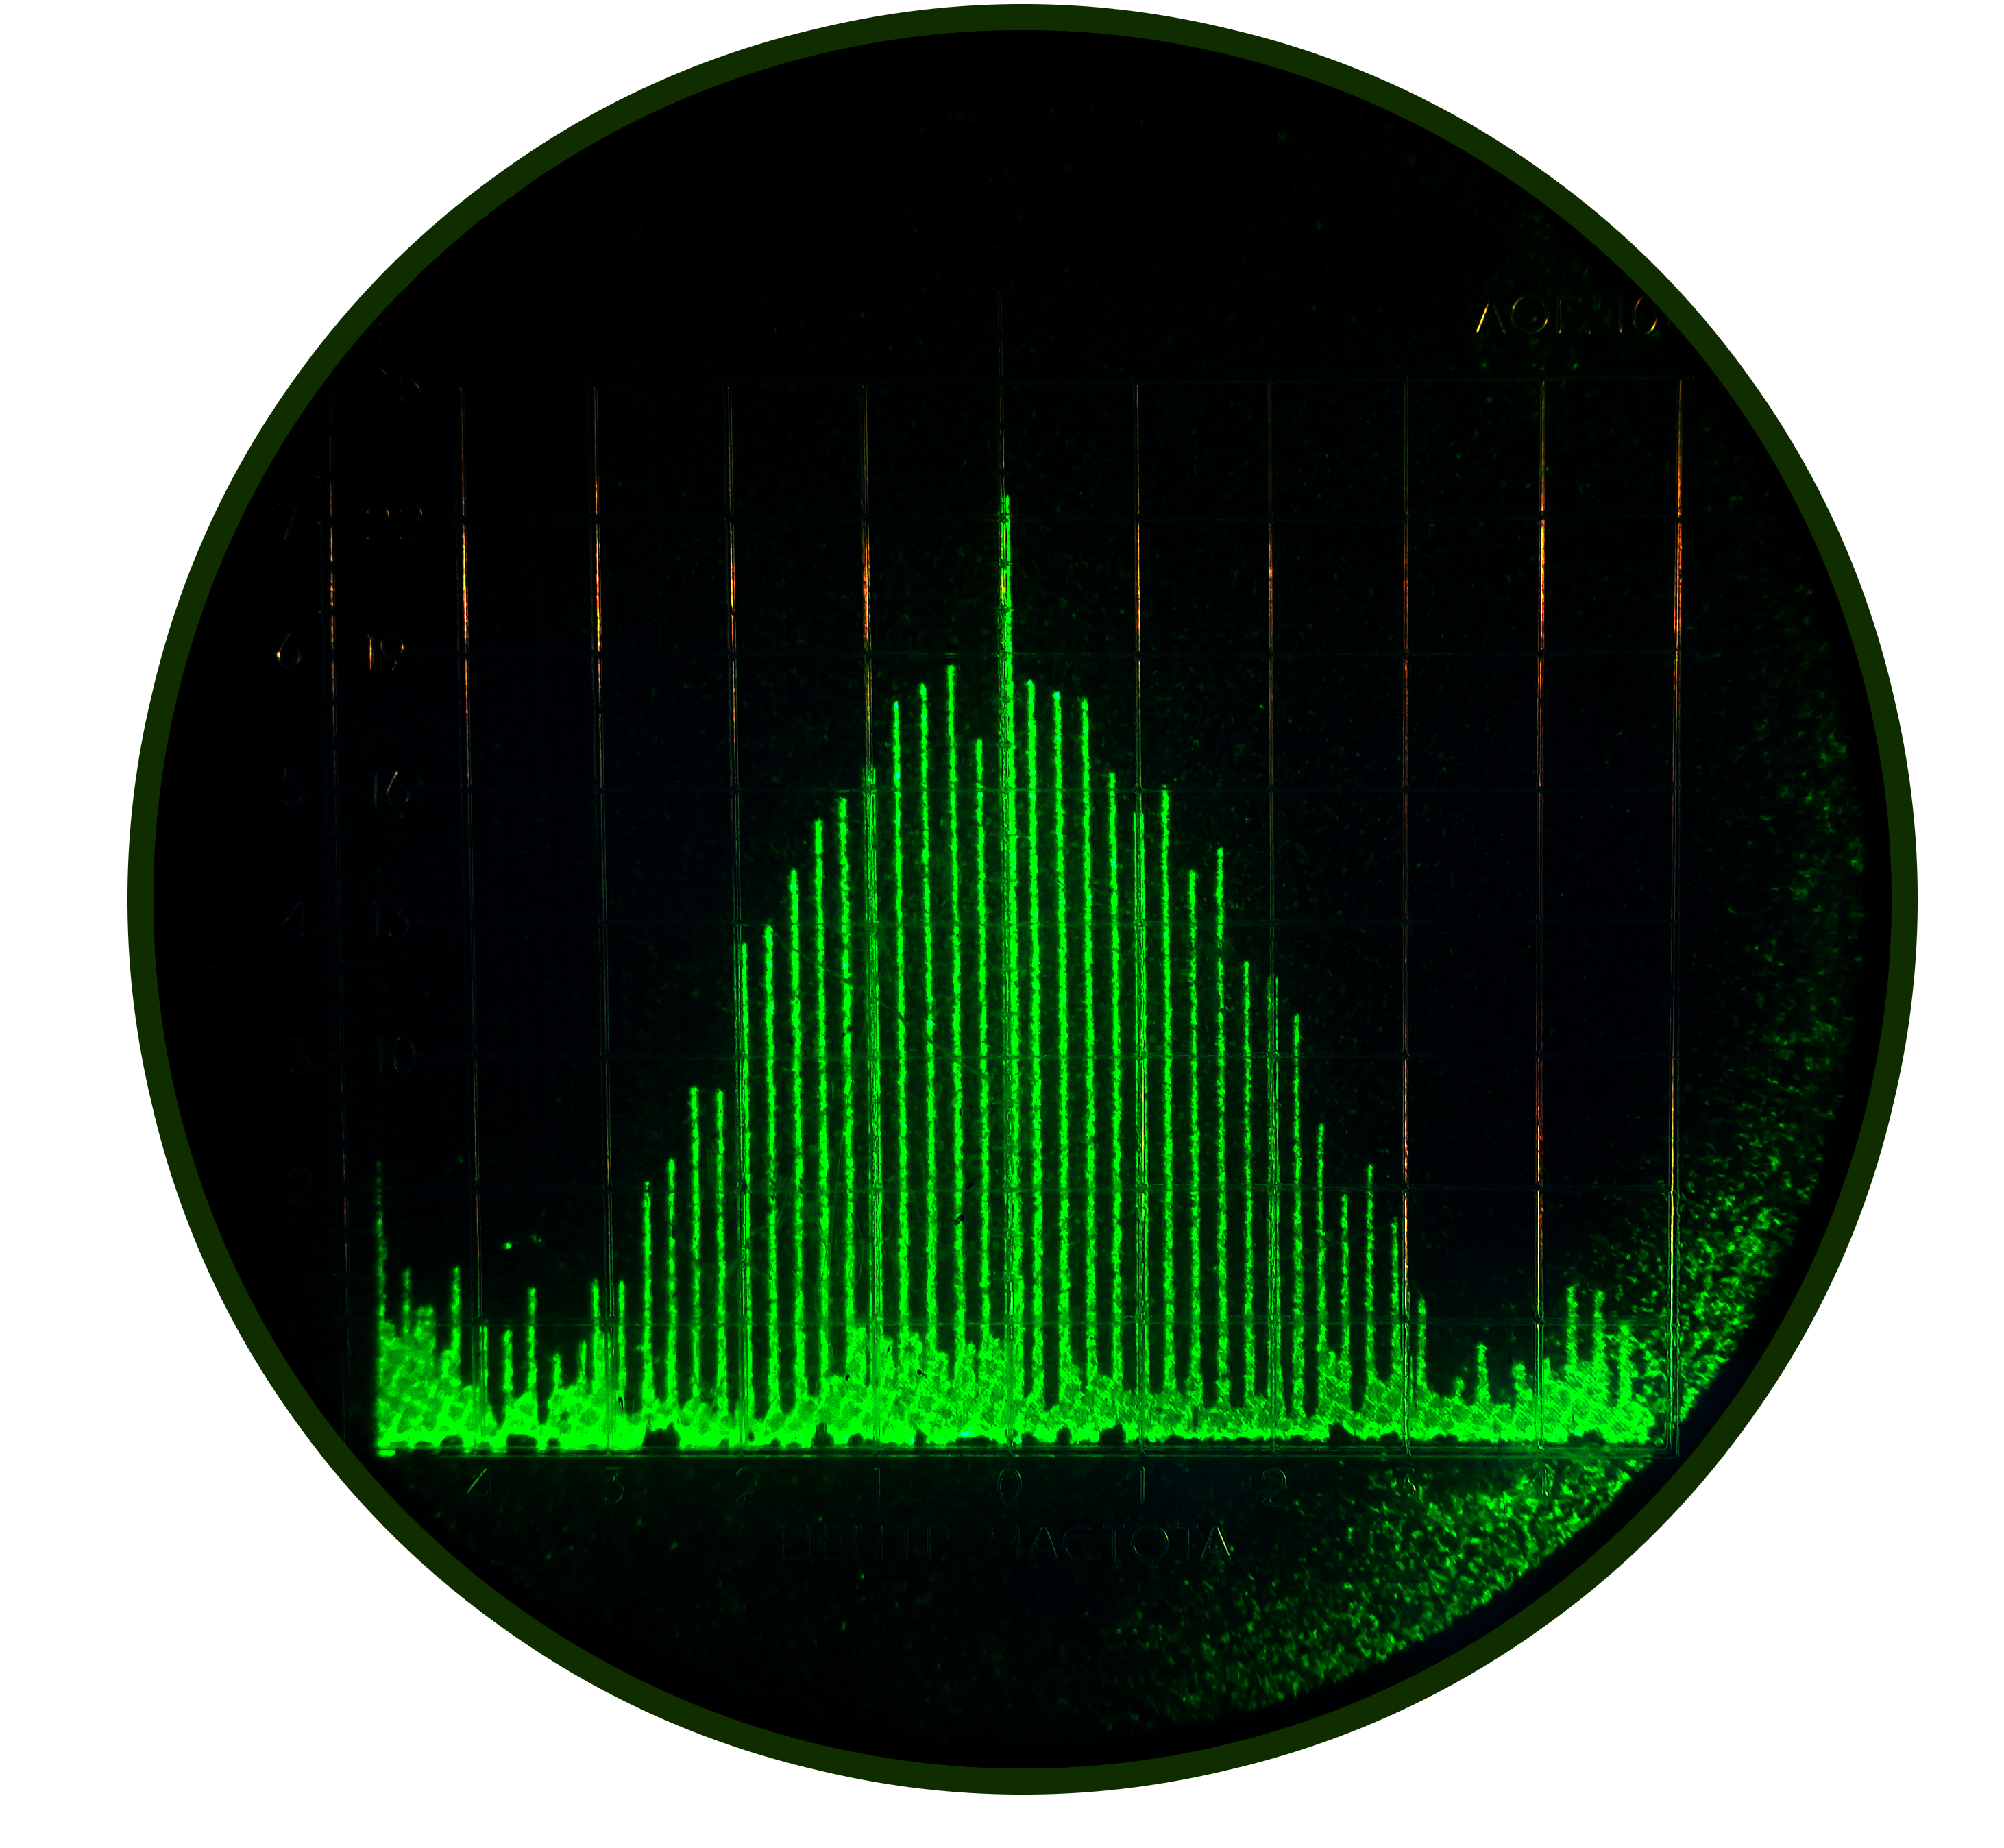
\includegraphics[width=0.9\linewidth]{50ex} \\ $\tau = 50$ мкс}
\end{minipage}
\hfill
\begin{minipage}[h]{0.49\linewidth}
\center{\includegraphics[width=0.9\linewidth]{100ex} \\ $\tau = 100$ мкс}
\end{minipage}
\caption{Спектры колебаний с различными параметрами длительности импульса}
\label{ris:image1}
\end{figure}


\subsection*{Исследование спектра гармонических сигналов, модулированных по амплитуде}

Рассмотрим гармонические колебания высокой частоты $\omega_0$, амплитуда которых, в свою очередь, меняется по гармоническому закону с частотой $\Omega \ll \omega_0$.

\begin{equation}
\label{form:amf(t)_a_n}
	f(t) = A_0[1+m\cos(\Omega t)]\cos(\omega_0t)
\end{equation}

Коэффициент $m$ - глубина модуляции и по определению:
\begin{equation}
\label{form:m}
	m = \frac{A_{max}-A_{min}}{A_{max}+A_{min}}
\end{equation}

\subsubsection*{Работа}
В работе используются: \textit{анализатор спектра СК4-56; генератор прямоугольных импульсов Г5-54; осциллограф; генератор сигналов Г6-34}

\begin{figure}[H]
\centering
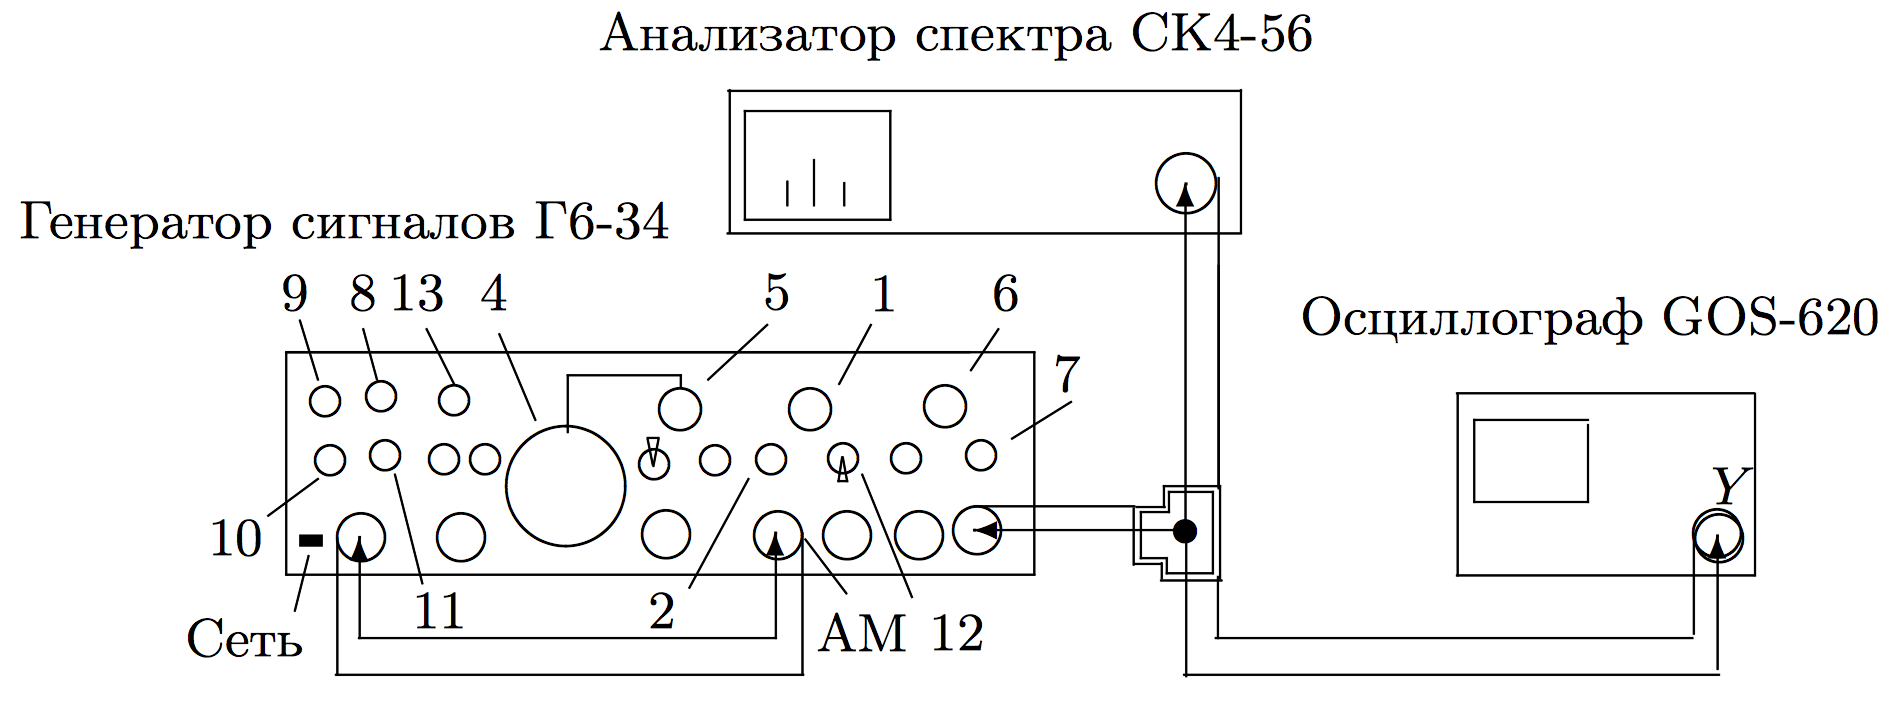
\includegraphics[width = 0.8\textwidth]{SchemeC}
\caption{Схема для исследования спектра гармонических сигналов, модулированных по амплитуде}
\label{img:scheme C}
\end{figure}

Собираем схему согласно \ref{img:scheme C}. Получаем на экране осциллографа гармонический сигнал, модулированный по амплитуде. Подключаем анализатор спектра СК4-56 и после настройки наблюдаем спектр сигнала.

Чтобы измерить глубину модуляции, измерим $A_{max}$, $A_{min}$ и подставим в формулу \ref{form:m}. Построим график отношения $a_\text{бок}/a_\text{осн}$ в зависимости от $m$.

Рассчитаем теоретический коэффициент наклона, воспользовавшись формулой:
\begin{equation}
\label{form:a/a(m)}
	f(t)=A_0\cos(\omega_0t)+	\frac{A_0m}{2}\cos(\omega_0+\Omega t)+\frac{A_0m}{2}\cos(\omega_0-\Omega t). 
\end{equation}

$$a_\text{осн} = A_0, \; a_\text{бок}= \frac{A_0m}{2} \Rightarrow k_\text{теор} = 0.5$$
	
\begin{table}[H]
\centering
\begin{tabular}{|l|l|l|l|l|l|}
\hline
\textbf{$2A_{max}$} & \textbf{$2A_{min}$} & \textbf{$a_\text{бок}$} & \textbf{$a_\text{осн}$} & \textbf{$m$} & \textbf{$a_\text{бок}/a_\text{осн}$} \\ \hline
5.4                 & 0.4                 & 4                       & 7.5                     & 0.53         & 0.86                                 \\ \hline
4.6                 & 1.2                 & 2.6                     & 7.7                     & 0.34         & 0.59                                 \\ \hline
4                   & 1.8                 & 1.7                     & 7.7                     & 0.22         & 0.38                                 \\ \hline
3.4                 & 2                   & 2.2                     & 7.6                     & 0.29         & 0.26                                 \\ \hline
3                   & 2.2                 & 0.6                     & 7.7                     & 0.08         & 0.15                                 \\ \hline
\end{tabular}
\caption{Экспериментальные данные}
\label{my-label}
\end{table}

\begin {figure}[H]
\begin{center}
{% GNUPLOT: LaTeX picture with Postscript
\begingroup
  \fontfamily{sansserif}%
  \selectfont
  \makeatletter
  \providecommand\color[2][]{%
    \GenericError{(gnuplot) \space\space\space\@spaces}{%
      Package color not loaded in conjunction with
      terminal option `colourtext'%
    }{See the gnuplot documentation for explanation.%
    }{Either use 'blacktext' in gnuplot or load the package
      color.sty in LaTeX.}%
    \renewcommand\color[2][]{}%
  }%
  \providecommand\includegraphics[2][]{%
    \GenericError{(gnuplot) \space\space\space\@spaces}{%
      Package graphicx or graphics not loaded%
    }{See the gnuplot documentation for explanation.%
    }{The gnuplot epslatex terminal needs graphicx.sty or graphics.sty.}%
    \renewcommand\includegraphics[2][]{}%
  }%
  \providecommand\rotatebox[2]{#2}%
  \@ifundefined{ifGPcolor}{%
    \newif\ifGPcolor
    \GPcolorfalse
  }{}%
  \@ifundefined{ifGPblacktext}{%
    \newif\ifGPblacktext
    \GPblacktexttrue
  }{}%
  % define a \g@addto@macro without @ in the name:
  \let\gplgaddtomacro\g@addto@macro
  % define empty templates for all commands taking text:
  \gdef\gplbacktext{}%
  \gdef\gplfronttext{}%
  \makeatother
  \ifGPblacktext
    % no textcolor at all
    \def\colorrgb#1{}%
    \def\colorgray#1{}%
  \else
    % gray or color?
    \ifGPcolor
      \def\colorrgb#1{\color[rgb]{#1}}%
      \def\colorgray#1{\color[gray]{#1}}%
      \expandafter\def\csname LTw\endcsname{\color{white}}%
      \expandafter\def\csname LTb\endcsname{\color{black}}%
      \expandafter\def\csname LTa\endcsname{\color{black}}%
      \expandafter\def\csname LT0\endcsname{\color[rgb]{1,0,0}}%
      \expandafter\def\csname LT1\endcsname{\color[rgb]{0,1,0}}%
      \expandafter\def\csname LT2\endcsname{\color[rgb]{0,0,1}}%
      \expandafter\def\csname LT3\endcsname{\color[rgb]{1,0,1}}%
      \expandafter\def\csname LT4\endcsname{\color[rgb]{0,1,1}}%
      \expandafter\def\csname LT5\endcsname{\color[rgb]{1,1,0}}%
      \expandafter\def\csname LT6\endcsname{\color[rgb]{0,0,0}}%
      \expandafter\def\csname LT7\endcsname{\color[rgb]{1,0.3,0}}%
      \expandafter\def\csname LT8\endcsname{\color[rgb]{0.5,0.5,0.5}}%
    \else
      % gray
      \def\colorrgb#1{\color{black}}%
      \def\colorgray#1{\color[gray]{#1}}%
      \expandafter\def\csname LTw\endcsname{\color{white}}%
      \expandafter\def\csname LTb\endcsname{\color{black}}%
      \expandafter\def\csname LTa\endcsname{\color{black}}%
      \expandafter\def\csname LT0\endcsname{\color{black}}%
      \expandafter\def\csname LT1\endcsname{\color{black}}%
      \expandafter\def\csname LT2\endcsname{\color{black}}%
      \expandafter\def\csname LT3\endcsname{\color{black}}%
      \expandafter\def\csname LT4\endcsname{\color{black}}%
      \expandafter\def\csname LT5\endcsname{\color{black}}%
      \expandafter\def\csname LT6\endcsname{\color{black}}%
      \expandafter\def\csname LT7\endcsname{\color{black}}%
      \expandafter\def\csname LT8\endcsname{\color{black}}%
    \fi
  \fi
    \setlength{\unitlength}{0.0500bp}%
    \ifx\gptboxheight\undefined%
      \newlength{\gptboxheight}%
      \newlength{\gptboxwidth}%
      \newsavebox{\gptboxtext}%
    \fi%
    \setlength{\fboxrule}{0.5pt}%
    \setlength{\fboxsep}{1pt}%
\begin{picture}(9354.00,6802.00)%
    \gplgaddtomacro\gplbacktext{%
      \csname LTb\endcsname%
      \put(660,1408){\makebox(0,0)[r]{\strut{}$0$}}%
      \csname LTb\endcsname%
      \put(660,2219){\makebox(0,0)[r]{\strut{}$0.1$}}%
      \csname LTb\endcsname%
      \put(660,3030){\makebox(0,0)[r]{\strut{}$0.2$}}%
      \csname LTb\endcsname%
      \put(660,3841){\makebox(0,0)[r]{\strut{}$0.3$}}%
      \csname LTb\endcsname%
      \put(660,4651){\makebox(0,0)[r]{\strut{}$0.4$}}%
      \csname LTb\endcsname%
      \put(660,5462){\makebox(0,0)[r]{\strut{}$0.5$}}%
      \csname LTb\endcsname%
      \put(660,6273){\makebox(0,0)[r]{\strut{}$0.6$}}%
      \csname LTb\endcsname%
      \put(924,968){\makebox(0,0){\strut{}$0$}}%
      \csname LTb\endcsname%
      \put(2604,968){\makebox(0,0){\strut{}$0.2$}}%
      \csname LTb\endcsname%
      \put(4285,968){\makebox(0,0){\strut{}$0.4$}}%
      \csname LTb\endcsname%
      \put(5965,968){\makebox(0,0){\strut{}$0.6$}}%
      \csname LTb\endcsname%
      \put(7646,968){\makebox(0,0){\strut{}$0.8$}}%
      \csname LTb\endcsname%
      \put(9326,968){\makebox(0,0){\strut{}$1$}}%
      \put(1764,5787){\makebox(0,0)[l]{\strut{}$K = \left(0.55\pm0.13\right)$ }}%
    }%
    \gplgaddtomacro\gplfronttext{%
      \csname LTb\endcsname%
      \put(-220,3840){\rotatebox{-270}{\makebox(0,0){\strut{}$\frac{a_\text{бок}}{a_\text{осн}}$}}}%
      \put(5125,308){\makebox(0,0){\strut{}$m$}}%
    }%
    \gplbacktext
    \put(0,0){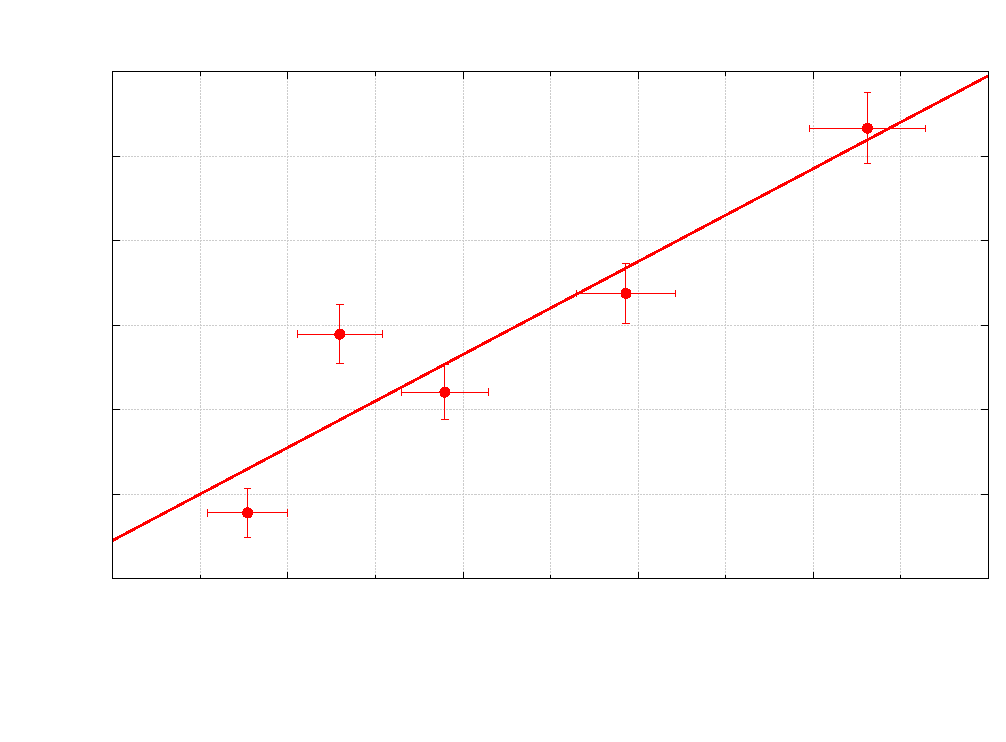
\includegraphics{magn}}%
    \gplfronttext
  \end{picture}%
\endgroup
}
\caption{График зависимости $\dfrac{a_\text{бок}}{a_\text{осн}}(m)$}
\end{center}
\end{figure}



Коэффициент угла наклона прямой и его погрешность посчитаем методом наименьших квадратов: $K = \left(0.55\pm0.13\right)$

\section{Вывод}

Экспериментально было проверено соотношение неопределенности в первых двух экспериментах. Точность достаточно высокая, полученные значения соответствуют ожиданиям. Основной вклад в погрешность вносит отсутствие мелких делений на анализаторе спектра.

В третьем эксперименте было проверена зависимость отношения амплитуд спектральных линий синусоидального сигнала, модулированного низкочастотными гармоническими колебаниями, от коэффициента модуляции.
\end{document}